\documentclass[conference]{IEEEtran}
\IEEEoverridecommandlockouts
\usepackage{cite}
\usepackage{amsmath,amssymb}
\usepackage{booktabs}
\usepackage{graphicx}
\usepackage[table]{xcolor}
\usepackage{url}
\usepackage{cuted}
\usepackage{capt-of}
\usepackage{dblfloatfix}
\usepackage[hidelinks,pdfauthor={},pdfcreator={},pdfproducer={}]{hyperref}
\newif\ifanonymous
\anonymoustrue   % set \anonymousfalse for the camera-ready / single-blind version
\newif\ifappendix
\appendixfalse   % set \appendixfalse if the venue counts appendices toward the page limit
\newcommand{\confirm}[1]{\textcolor{red}{[#1]}}
\newcommand{\artifact}{\ifanonymous\url{https://anonymous.4open.science/r/XXXXXXXX}\else\confirm{public repository URL}\fi}

\begin{document}

\title{HoNE: Does Hold-out Evidence Predict Natural Novelty? Testing the Protocol Validity of Zero-Day NIDS Evaluation}

\ifanonymous
\author{\IEEEauthorblockN{Anonymous Author(s)}\IEEEauthorblockA{Submission under double-blind review}}
\else
\author{\IEEEauthorblockN{Gracious Mwamughunda, Guohao Sun, Hafsa Aslam, Oussama Rizkou}
\IEEEauthorblockA{Donghua University, Shanghai, China\\
Email: 324078@mail.dhu.edu.cn, ghsun@dhu.edu.cn, 324091@mail.dhu.edu.cn, 324047@mail.dhu.edu.cn}}
\fi

\maketitle

\begin{abstract}
Learned network intrusion detection systems (NIDS) are adopted for their claimed ability to detect zero-day attacks, and operators must decide before deployment whether to trust that claim. The evidence offered is almost always leave-one-attack-class-out (LOACO) evaluation: one attack class is withheld from a randomly split benchmark and the detector is scored once by the area under the ROC curve (AUC). LOACO assumes that a withheld class stands for attacks that emerge later in time amid drifting benign traffic, but this assumption has not been tested. HoNE (Hold-out and Natural-novelty Evaluation) is a pre-registered, leakage-controlled paired methodology that scores the same detectors, data, backbones and seeds under LOACO and under natural novelty, where attack classes first appear after the training period, and measures their agreement, seed variability and detection at an operating point. On four NetFlow-v3 datasets and Lycos2017, 12 detectors on two recurrent backbones, five seeds and four rolling cut-offs (210 runs), LOACO is not a reliable proxy. Temporal LOACO cannot be run on day-scheduled captures; across 12 paired comparisons the best detector changes in 11 and rankings correlate with a median Spearman $\rho$ of 0.55, although the leading family within a dataset is preserved. Natural novelty raises seed-to-seed variation up to 17-fold, and family AUCs up to 0.75 catch at most 18\% of new attacks at a 1\% false-alarm rate. We turn each failure into one of eight acceptance checks an operator can require.
\end{abstract}

\begin{IEEEkeywords}
network intrusion detection, network security management, zero-day attacks, evaluation methodology, NetFlow
\end{IEEEkeywords}

\section{Introduction}
\label{sec:intro}
Network operators increasingly deploy machine-learning network intrusion detection systems (NIDS) because signature rules cannot cover attacks that did not exist when the rules were written. Consider an operator choosing between two learned detectors for an enterprise or IoT network. Both report high zero-day scores on public benchmarks; the operator deploys the better one, and months later a new attack class appears amid benign traffic that has changed since training. Whether the detector catches it depends on whether the benchmark evidence predicted exactly this situation.

The stakes are operational. An overstated detector misses the attacks it was bought to catch, and one whose performance varies between training runs gives no stable basis for alert thresholds or for staffing alert triage. Both surface only after deployment, so the validity of pre-deployment evidence is a network-management question, not only a machine-learning one.

The standard evidence for zero-day ability is \emph{leave-one-attack-class-out} (LOACO) evaluation: one attack class is withheld from training on a benchmark split at random, and the detector must flag it at test time~\cite{wilkie2026}. It is attractive because it runs on any labelled dataset and isolates a single unseen class, and it underlies the zero-day studies we review (Sec.~\ref{sec:related}).

LOACO, however, rests on assumptions that naturally emerging attacks do not satisfy. Random splits let near-identical flows and whole attack episodes appear in both training and test sets~\cite{arp2022}. LOACO keeps the benign traffic of the test period in training, so the withheld class is the only thing that changes, whereas a real new attack arrives \emph{later in time} alongside drifting benign traffic, which we call \emph{natural temporal novelty}. Results usually come from one run, are summarized by AUC, and often score novelty with confidence measures designed for multi-class image recognition~\cite{hendrycks2017,liu2020energy}. Such benchmark scores are known to overstate field performance~\cite{sommer2010,apruzzese2023sok}, yet whether LOACO conclusions transfer to natural novelty, a property we call \emph{protocol validity}, has not been measured: recent studies combine time-ordered splits with held-out attack families~\cite{nayak2026,alhalangy2026} or compare several protocols~\cite{mesca2026,raj2026}, but to evaluate a proposed detector rather than to test the protocol itself.

This paper therefore asks one question: \emph{can hold-out zero-day evidence predict natural novelty?} It has two parts. First, does LOACO evidence \emph{agree} with natural novelty: can it be produced on time-ordered captures, and does it select the same detectors, rankings and AUC levels? Second, what does hold-out evidence \emph{hide}, in run-to-run variability and in detection at the false-alarm rate an operator can absorb?

We answer it with \textbf{HoNE} (\textbf{Ho}ld-out and \textbf{N}atural-novelty \textbf{E}valuation), a paired methodology that treats the evaluation protocol, not the detector, as the object of study (Fig.~\ref{fig:overview}). HoNE builds leakage-controlled splits from flow timestamps and scores every detector under both protocols on the same data, backbones and five seeds. It then measures agreement (rank correlation, change of best detector, AUC and TPR differences), seed variability and operating-point detection, and checks them with stress and validity tests: purged-block LOACO, rolling training cut-offs, in-distribution temporal shift, cross-network transfer and a second backbone. All hypotheses were hashed before each experiment, and failed ones are reported (Sec.~\ref{sec:neg}).

Applied to five public datasets and 12 detectors, HoNE shows that \emph{conventional hold-out evaluation is not a reliable proxy for natural attack emergence}. Temporal LOACO cannot be run on any day-scheduled capture (Sec.~\ref{sec:c1}). Where both protocols run, LOACO preserves the leading detector family within a dataset, but the best detector changes in 11 of 12 paired comparisons and rankings agree only moderately (median $\rho{=}0.55$; Sec.~\ref{sec:c2}). Natural novelty exposes instability that LOACO hides: seed variation rises up to 17$\times$ (2.6$\times$ on the second backbone; Sec.~\ref{sec:c3}). Neither inverted confidence scores nor temporal shift alone explains the disagreement (Secs.~\ref{sec:c4}--\ref{sec:c5}), and the gap matters at the operating point: family AUCs up to 0.75 catch at most 18\% of new attacks at a 1\% false-alarm rate (Sec.~\ref{sec:c6}).

These findings define what credible zero-day evidence must contain: each exposes a failure mode, and each failure mode yields a check an operator can require. Because the best detector changes with the protocol, a LOACO-only result cannot select a detector, so natural-novelty results are required wherever timestamps allow. Because seed variation hides under LOACO, a single run can misrank detectors, so five or more seeds with per-class spread are required. Because AUC hides missed attacks, detection at the operator's false-positive rate is required. The resulting \emph{HoNE acceptance protocol} has eight such checks (Sec.~\ref{sec:disc}), each cheap: one of our runs takes about three CPU-minutes.

Our key contributions are:
\begin{itemize}
\item a paired, pre-registered methodology that tests the protocol validity of zero-day NIDS evidence (Sec.~\ref{sec:method});
\item a quantification of LOACO--natural-novelty disagreement in feasibility, detector choice, rankings and AUC (Secs.~\ref{sec:c1}, \ref{sec:c2}, \ref{sec:c5});
\item evidence that hold-out evaluation hides seed instability and overstates operating-point detection (Secs.~\ref{sec:c3}, \ref{sec:c6}), and that MSP and energy invert in binary detectors (Sec.~\ref{sec:c4});
\item an eight-check acceptance protocol derived from these findings (Sec.~\ref{sec:disc}).
\end{itemize}

\section{Related Work}
\label{sec:related}
Prior work on learned NIDS evaluation falls into five lines, each leaving a different piece of what an operator needs missing.

\textbf{Evaluation pitfalls and datasets.} Arp et~al.\ catalogued ten pitfalls in security ML, including data snooping and inappropriate baselines~\cite{arp2022}; Apruzzese et~al.\ showed that ML-NIDS evaluations rarely reflect operational assumptions~\cite{apruzzese2023sok}; and dataset audits found flow-construction and labelling errors in CIC-IDS2017~\cite{engelen2021,rosay2021} and Pinto et~al.\ reviewed the tools and processes used to build NIDS datasets and their drawbacks~\cite{pinto2025}. The NetFlow standardization of Sarhan et~al.\ made datasets comparable~\cite{sarhan2021netflow,sarhan2022standard}, and its third version adds per-flow timestamps~\cite{luay2025}. These works diagnose \emph{how} evaluations go wrong, but they do not compare zero-day protocols or measure what the pitfalls do to detector rankings.

\textbf{Zero-day and open-set detection.} Zoppi et~al.\ found that unsupervised meta-learning ensembles detect simulated unknown attacks better than other algorithm families~\cite{zoppi2023}, and Sarhan et~al.\ linked low zero-day detection rates to distribution distance~\cite{sarhan2023zeroshot}. Recent detectors train with known attacks, via a contrastive loss (CLAD~\cite{wilkie2026}) or a transformer with energy scoring~\cite{jodayree2026}. These studies measure zero-day ability, but all of them use class hold-out, usually without reporting seed variability, so their conclusions inherit LOACO's assumptions.

\textbf{Temporal and protocol-aware evaluation.} Time-aware evaluation changed conclusions in malware detection~\cite{pendlebury2019} and intrusion detection under drift~\cite{andresini2021}, and multi-period benchmarks such as AnoShift~\cite{dragoi2022} and MAWIFlow~\cite{schraven2026} test detectors on traffic from later years. For zero-day detection, ThreatFormer-IDS splits ToN-IoT in time and then removes chosen attack families from training, reporting five seeds and recall at 1\% FPR for a single model~\cite{nayak2026}; Alhalangy and Eltayeb combine chronological splits with leave-one-attack-family-out for one proposed detector~\cite{alhalangy2026}; Mesca et~al.\ compare random, attack-held-out and leave-one-out protocols on industrial traffic~\cite{mesca2026}; and Raj et~al.\ report future-time and leave-one-attack-type-out tests on RPL-IoT~\cite{raj2026}. Chronological splits on day-scheduled CIC-IDS2017 degenerate~\cite{moczkodan2026}, capture-day assembly~\cite{youssef2026} and temporal splits~\cite{abdessamad2026} change detector rankings, and timestamps leak the attack schedule~\cite{sakr2026}. These studies vary the protocol to test a detector; HoNE holds the detectors fixed and varies the protocol, including seed variability and a moving training origin.

\textbf{Confidence scores for unknown attacks.} Confidence-based out-of-distribution scores are weaker on binary than on multi-class NIDS models~\cite{corsini2023}, softmax baselines scored below chance on held-out attacks in multi-class NIDS~\cite{zhang2021}, softmax entropy and energy trailed uncertainty-aware models~\cite{talpini2024}, and deep open-set recognition has been benchmarked for NIDS at NOMS~\cite{baye2023}. In contrast to Mesca et~al., who sign-flip ensemble members whose attack probability falls below chance~\cite{mesca2026}, we find the attack probability valid and MSP and energy inverted, and give a short derivation of why.

\textbf{Cross-domain generalization.} Layeghy and Portmann~\cite{layeghy2023xdomain}, DI-NIDS~\cite{layeghy2023dinids}, Cantone et~al.~\cite{cantone2024} and recent work on flow-based IoT detection~\cite{martinez2026} show that detectors degrade sharply on networks other than the one they were trained on. This line addresses shift \emph{between} networks, whereas an operator's first concern is shift \emph{over time within} the network being protected.

\textbf{Research gap and positioning.} Taken together, these lines leave the protocol validity of zero-day evidence untested; HoNE tests it by scoring the same detectors, data and seeds under both protocols.\ifappendix\ Appendix~\ref{app:related} extends this review to sequence, neuromorphic and drift-aware NIDS and positions HoNE against prior work in Table~\ref{tab:pos}.\fi

\section{Methodology}
\label{sec:method}
HoNE takes public flow datasets with per-flow timestamps and a panel of detectors, and determines whether zero-day evidence obtained under class hold-out agrees with detector behaviour under natural temporal novelty. As summarized in Fig.~\ref{fig:overview}, the methodology proceeds from these inputs through four stages. Section~\ref{sec:data} describes the input data; Section~\ref{sec:s1} (Stage~1) removes leakage and produces clean windows; Section~\ref{sec:s2} (Stage~2) splits them under paired zero-day protocols; Section~\ref{sec:s3} (Stage~3) trains and scores the detector panel over several seeds; and Section~\ref{sec:prereg} (Stage~4) turns the scores into metrics, findings and an acceptance decision. Together, these stages specify the complete path from raw flow records to an evidence-based decision on a zero-day claim.

\begin{figure*}[!t]
    \centering
    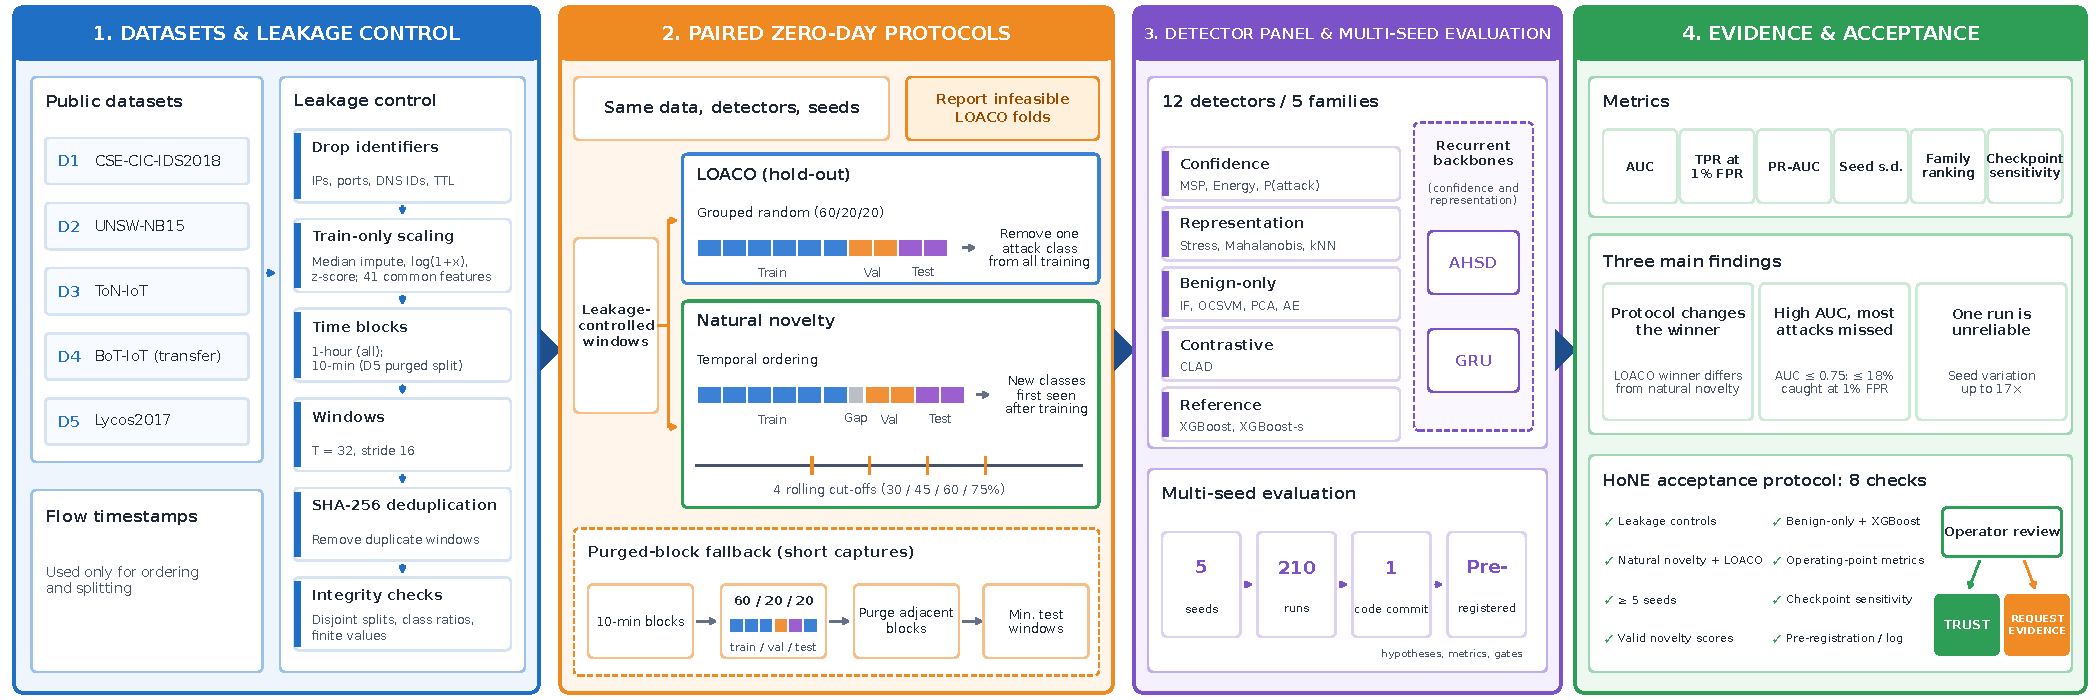
\includegraphics[width=\textwidth]{fig_methodology.pdf}
    \caption{HoNE methodology: (1) datasets and leakage control, (2) paired zero-day protocols on the same data, shown on a toy capture, (3) the same detector panel and five seeds under both protocols, and (4) paired evidence (agreement, seed variability, operating point) and acceptance.}
    \label{fig:overview}
\end{figure*}




\subsection{Input data}
\label{sec:data}
\textbf{Input data.} HoNE takes public flow-level datasets with per-flow timestamps as input~\cite{sarhan2021netflow,luay2025}. D1--D4 are the NetFlow-v3 versions of CSE-CIC-IDS2018~\cite{sharafaldin2018}, UNSW-NB15~\cite{moustafa2015}, ToN-IoT~\cite{moustafa2021} and BoT-IoT~\cite{koroniotis2019}, which share 53 features~\cite{luay2025}; D5 is Lycos2017, a corrected re-extraction of CIC-IDS2017~\cite{sharafaldin2018} that fixes documented flow-construction and labelling errors~\cite{engelen2021,rosay2021}, processed in its own feature space (Table~\ref{tab:data}). Every flow carries a binary label and an attack-class label~\cite{sarhan2021netflow,sarhan2022standard}. For D1--D4 the dataset maintainers re-extracted each testbed's packet captures into this common NetFlow schema with millisecond start and end timestamps~\cite{sarhan2021netflow}, which makes strictly time-ordered splits possible; for D5 we run the authors' labelling script unmodified and map its timestamps and labels to the same fields. All files come from the official sources, are registered with their SHA-256 and row count, and are audited for schema conformity, missing and infinite values, label consistency and timestamp range before use; they are never modified. D4, whose capture is dominated by attack traffic~\cite{koroniotis2019}, contains only 1,315 benign windows and serves only as a transfer target, and D1's 14 file labels are grouped into six attack families matching the attack scenarios of the original capture~\cite{sharafaldin2018}, so that a held-out class has no near-identical sibling in training.

\begin{center}
\scriptsize
\setlength{\tabcolsep}{3pt}

\captionof{table}{Datasets. Windows are counted before deduplication.}
\label{tab:data}

\begin{tabular}{llrrrl}
\toprule
ID & Dataset & Flows & Windows & Dupl. & Classes\\
\midrule
D1 & NF-CIC-IDS2018-v3 & 20.1\,M & 1,257,018 & 1,838 & 14 (6 fam.)\\
D2 & NF-UNSW-NB15-v3 & 2.37\,M & 147,801 & 0 & 9\\
D3 & NF-ToN-IoT-v3 & 27.5\,M & 1,719,860 & 166,669 & 9\\
D4 & NF-BoT-IoT-v3 & 16.9\,M & 890,852$^{a}$ & -- & 4\\
D5 & Lycos2017 & 1.84\,M & 114,783 & 0 & 13\\
\bottomrule
\multicolumn{6}{l}{$^{a}$Windows retained; D4 has no split of its own (transfer target only).}
\end{tabular}
\end{center}

\subsection{Stage 1: Leakage control}
\label{sec:s1}
Stage~1 turns raw flows into windows that cannot leak information between training and test sets. Addresses, ports and DNS query IDs are dropped, and TTL fields are dropped as a known UNSW-NB15 label-leakage artifact; flow timestamps are kept only for ordering and splitting. Infinite values are imputed with the training median, heavy-tailed counts are $\log(1{+}x)$-transformed, and features are standardized with training statistics, leaving 41 common features over D1--D3. Flows are then sorted by start time and grouped into 1-hour blocks (10-minute blocks for D5's purged split) \emph{before} windowing into $T{=}32$ flows with stride 16, so that no window crosses a block. A window is an attack if any flow is, and its class is the majority attack class. Windows are hashed and exact duplicates removed globally, which removed 9.7\% of D3's windows.

Because a silent leakage bug would invalidate every later result, each build ends with fail-closed integrity checks covering hash- and block-level disjointness of splits, class ratios, the absence of held-out flows from LOACO training sets, and finite values. All passed, including 538 checks on the D1--D4 archives after Amendment~1 and 32 on the D5 purged-block build. The output of Stage~1 is a set of leakage-controlled windows per dataset.

\subsection{Stage 2: Paired zero-day protocols}
\label{sec:s2}
Stage~2 derives every zero-day evaluation from two splits of the same windows. \emph{grouped\_random} shuffles blocks 60/20/20 into training, validation and test sets, and \emph{temporal\_gap} orders them in time, with the first 60\% for training, one discarded gap block, then 20\% each for validation and test (Fig.~\ref{fig:overview}, panel~2). The evaluations form two levels. The \emph{primary paired comparison} scores every detector under (1)~LOACO and (2)~natural novelty. Four \emph{additional validity and stress evaluations} test that comparison: (3)~purged-block LOACO for the short D5 capture, (4)~rolling natural novelty, (5)~in-distribution AUC on the grouped and temporal splits, which isolates temporal shift without novelty, and (6)~zero-shot transfer of D1--D3 models to the other datasets.
\begin{itemize}
\item (1)~\emph{LOACO} runs on grouped\_random: one attack class is removed from training and tested on. A class is eligible if its training pool holds at least 200 windows (by majority label), and it is evaluated only if it also occurs in the test split.
\item (2)~\emph{Natural novelty} runs on temporal\_gap and scores the classes that occur in test but never in training; its validation set is the last 20\% of the training period.
\item (4)~\emph{Rolling cut-points} (Amendment~7) re-apply the natural-novelty rule with the training period ending at 30, 45, 60 and 75\% of each dataset's windows, one discarded gap block, and testing on everything after; the cleaner is refitted on each cut's training rows, and each (dataset, cut, class) is one class--cut unit.
\item (3)~\emph{Purged blocks}, for short captures, assign 10-minute blocks 60/20/20 within each capture day and remove blocks adjacent to test or validation blocks, following purged cross-validation~\cite{lopezdeprado2018}; folds additionally require 50 test windows.
\end{itemize}
Training sets are balanced 1:1 (7,000 windows per class), and validation and test sets use a 5:1 benign-to-attack ratio. Protocols that cannot be run on a dataset are reported rather than skipped. The output of Stage~2 is one set of training, validation and test windows per dataset and protocol, shared by every detector.

\subsection{Stage 3: Detector panel and multi-seed runs}
\label{sec:s3}
Stage~3 trains and scores every detector on every split from Stage~2. HoNE groups 12 scores into five families by what they read from a model, adapted from the taxonomy of~\cite{yang2024ood} (Table~\ref{tab:det}). \emph{Confidence} scores read the classifier output; \emph{representation-distance} scores read hidden features~\cite{lee2018,sun2022knn}; \emph{benign-only} detectors never see attacks~\cite{liu2008,scholkopf2001}; the \emph{contrastive} detector CLAD~\cite{wilkie2026} is trained on benign and known attacks; and XGBoost~\cite{chen2016} on flattened windows is a supervised reference. Higher scores always mean more anomalous, and orientation was fixed before any run.

\makeatletter
\begin{center}
\scriptsize
\setlength{\tabcolsep}{2.5pt}

\def\@captype{table}
\caption{Twelve detectors in five families, plus a seeded XGBoost-s; confidence and representation scores are also computed on a GRU backbone.}
\label{tab:det}

\begin{tabular}{lll}
\toprule
Family & Detectors & Fitted on\\
\midrule
Confidence & MSP~\cite{hendrycks2017}, Energy~\cite{liu2020energy}, $P(\text{attack})^\dagger$ & Backbone output\\
Representation & Stress, Mahalanobis~\cite{lee2018}, $k$NN~\cite{sun2022knn} & Backbone features\\
Benign-only & IF~\cite{liu2008}, OCSVM~\cite{scholkopf2001}, PCA, autoencoder & Benign windows\\
Contrastive & CLAD~\cite{wilkie2026} & Benign + attacks\\
Reference & XGBoost~\cite{chen2016}, XGBoost-s & Labelled windows\\
\bottomrule
\end{tabular}
\end{center}
\makeatother

Confidence and representation scores come from a recurrent backbone (AHSD) built around a fixed benign reference $E$. Each flow vector is embedded as $z_t=\mathrm{LayerNorm}(Wx_t)\in\mathbb{R}^{128}$, and a state $h_t$, initialised at $E$, tracks the input relative to it with per-step, per-channel gates:
\begin{equation}
h_t = h_{t-1} + \alpha_t\odot(z_t - E) - \beta_t\odot(h_{t-1}-E),
\end{equation}
with gates $[\alpha_t,\beta_t]=\sigma(W_g[z_t,h_{t-1}])$. $E$ is not learned: it is the mean embedding of benign training windows, tracked by an exponential moving average during training and set exactly afterwards. Stress $=\frac{1}{TD}\sum_{t,d}|h_{t,d}-E_d|$, and a two-layer head (linear--GELU--linear) reads $[h_T,\ \frac{1}{T}\sum_t h_t,\ \text{stress}]$ and outputs $P(\text{attack})$; its hidden layer is the representation used by Mahalanobis and $k$NN. To test whether findings depend on this backbone, every confidence and representation score is recomputed on a second backbone, a one-layer GRU (hidden size 128) with the same embedding and head (without stress), trained identically (Amendment~7). XGBoost uses subsample and column sampling of 1 and is therefore deterministic; XGBoost-s uses 0.8 for both with the run's seed, so that the stability comparison is not made against a deterministic baseline.

Confidence scores need care in a binary detector. With logit margin $\Delta=f_{\text{attack}}-f_{\text{benign}}$, MSP $=\max(P(\text{attack}),\,1-P(\text{attack}))=\sigma(|\Delta|)$ measures how \emph{sure} the model is, not \emph{which} class it chose; temperature calibration rescales $\Delta$ and cannot change this ranking. A new attack that the classifier detects confidently has MSP close to 1, so the anomaly score $1-\text{MSP}$ is close to 0 and the attack reads as in-distribution; energy behaves the same way because it decreases as the largest logit grows. HoNE therefore reports $P(\text{attack})$ alongside MSP and energy; because it was added after the final pre-registered gate (marked $\dagger$), comparisons involving it are diagnostic rather than confirmatory.

Every detector--split configuration is run with five seeds. To keep the pipeline accountable, research questions, metrics and gates were written to a file and hashed before each experiment, and every result records that hash, the code commit and the dataset hashes~\cite{nosek2018}. Seven dated amendments are recorded, each hashed before the runs it governed, and none changed a recorded verdict: Amendments~2--4 followed failed gates, Amendment~6 turned the study into a descriptive benchmark after the fourth, and Amendment~7 added the GRU backbone, XGBoost-s, rolling cut-points and operating-point metrics. The output of Stage~3 is one anomaly score per window, detector, split and seed.

\subsection{Stage 4: Evidence and acceptance}
\label{sec:prereg}
Stage~4 turns the scores into evidence an operator can act on. For every detector and class it computes ROC AUC, PR-AUC and the true-positive rate at 1\% false-positive rate (TPR@1\%), the quantity a security team experiences; the 1\% threshold is set on each test set's benign windows, so TPR@1\% is descriptive. Results are reported as the mean over seeds with a Student-$t$ 95\% interval and the seed standard deviation, so that run-to-run variation is visible rather than averaged away. Per family, HoNE averages over detectors and classes and attaches a paired bootstrap interval over classes and seeds (2,000 resamples), then ranks the families for each protocol. To measure protocol validity, HoNE compares each detector's mean AUC under the two protocols on the same dataset and backbone: the difference $\Delta\text{AUC}=\text{AUC}_{\text{natural}}-\text{AUC}_{\text{LOACO}}$ (and likewise for TPR@1\%), the Spearman rank correlation $\rho$ of the detectors, the share of detector pairs whose order reverses, and whether the best detector changes; this comparison was added after the runs and is descriptive. Every evaluation is repeated with the final-epoch checkpoint to measure checkpoint sensitivity. All intervals are descriptive. Finally, these results are condensed into the HoNE acceptance protocol (Sec.~\ref{sec:disc}): eight checks an operator can require, which lead either to trusting a zero-day claim or to requesting the missing evidence.

\section{Evaluation}
\label{sec:eval}
We use HoNE to answer six research questions, each of which tests one part of the central claim:
\begin{itemize}
\item \textbf{RQ1:} Can conventional zero-day evidence be produced on time-ordered captures? (Sec.~\ref{sec:c1})
\item \textbf{RQ2:} Does conventional zero-day evidence agree with natural novelty? (Sec.~\ref{sec:c2})
\item \textbf{RQ3:} Does natural novelty expose instability that hold-out evidence hides? (Sec.~\ref{sec:c3})
\item \textbf{RQ4:} Are confidence-based novelty scores valid in binary detectors? (Sec.~\ref{sec:c4})
\item \textbf{RQ5:} Does temporal shift alone explain the disagreement? (Sec.~\ref{sec:c5})
\item \textbf{RQ6:} Does AUC overstate operational detection? (Sec.~\ref{sec:c6})
\end{itemize}
RQ1 and RQ2 test protocol validity directly; RQ3 and RQ6 test what hold-out evidence hides; RQ4 and RQ5 rule out alternative explanations.

\subsection{Evaluation setup}
Both backbones are trained with AdamW (learning rate $10^{-3}$, weight decay $10^{-4}$), cosine annealing, gradient clipping at 1.0, batch size 256 and 15 epochs; the best validation macro-F1 checkpoint is kept (CLAD: best validation AUROC). Seeds are 17, 23, 42, 101 and 202, and a seeding regression test runs before every experiment. All 210 final runs (Amendment~7) used one code commit and include the 160 runs of Amendment~6, whose results they reproduce exactly; reports are regenerated from stored result files only. Compute: a CPU-only cloud container (4 vCPUs, Intel Xeon at 2.10\,GHz, no GPU); the 210 runs took 10.8\,h (185\,s per run, both backbones and all detectors).

\subsection{RQ1: Can conventional zero-day evidence be produced on time-ordered captures?}
\label{sec:c1}
The first question is whether the standard protocol can even be run once leakage is controlled. Temporal LOACO yields no feasible folds on any of the three day-scheduled captures (D1, D3, D5); only D2, which interleaves attacks in time, supports it (Table~\ref{tab:feas}). In D1 and D3 each attack class occupies its own days, so a time-ordered split places a class wholly in training or wholly in test. On D5 the purged split kept 125 of 219 blocks, and only one class (dos\_hulk) met both thresholds. Natural novelty, by contrast, offers two to five evaluable classes on every day-scheduled capture, and moving the cut-point multiplies this evidence to 45 class--cut units over 19 unique classes, 15 per dataset (D2 has no test-only class at any cut, and D3 no benign validation windows at a 30\% cut).

\textbf{Answer to RQ1.} No: temporal LOACO cannot be run on any day-scheduled capture, whereas natural novelty provides 45 class--cut units.

\begin{table}[!t]
\centering\footnotesize\setlength{\tabcolsep}{3pt}
\caption{Feasible zero-day evaluations per dataset (LOACO folds; natural-novelty classes; rolling class--cut units with feasible cuts out of 4).}
\label{tab:feas}
\begin{tabular}{lcccc}
\toprule
Dataset & Grouped & Temporal & Natural & Rolling\\
\midrule
D1 CIC-IDS2018 & 6 & 0 & 2 & 15 (4)\\
D2 UNSW-NB15 & 8 & 8 & 0 & 0 (0)\\
D3 ToN-IoT & 6 & 0 & 5 & 15 (3)\\
D5 Lycos2017 & 0$^{a}$ & 0 & 2 & 15 (3)\\
\midrule
\multicolumn{5}{l}{$^{a}$One fold under the purged-block split.}\\
\bottomrule
\end{tabular}
\end{table}

\subsection{RQ2: Does conventional zero-day evidence agree with natural novelty?}
\label{sec:c2}
Where both protocols run (D1, D3, D5), we pair each detector's mean AUC under LOACO with its mean AUC under natural novelty, per dataset, backbone (AHSD: 12 detectors; GRU: its five scores plus the six backbone-free detectors) and natural-novelty view (fixed split; rolling cuts pooled), giving 12 paired comparisons (Table~\ref{tab:agree}).

The protocols disagree at the level an operator acts on. The best single detector changes in 11 of 12 comparisons (D1: PCA under LOACO, Mahalanobis under natural novelty; D5: XGBoost, then a representation distance). Rank correlation between the protocols ranges from 0.26 to 0.92 (median 0.55), and 9--36\% of detector pairs reverse order. Natural novelty lowers mean AUC in 10 comparisons, by up to 0.197; single detectors move by up to 0.451, and 9 detector--comparison cells cross from one side of chance to the other. TPR@1\% differs by 0.10--0.32 on average. The three D3 classes evaluated under both protocols show the same pattern class by class ($\rho$ 0.55--0.85; the best detector changes in 3 of 6 class--backbone pairs; mean AUC lower in all six). What LOACO does preserve is the leading family within a dataset (no change in 12 comparisons): its signal is coarse, not detector-level.

Margins between families are not preserved either (Table~\ref{tab:fam}). On D3, benign-only and representation scores are close under LOACO ($+0.022$ [$+0.004$, $+0.047$]), whereas under natural novelty benign-only detectors lead by $+0.376$ [$+0.247$, $+0.500$] and representation scores fall to chance. CLAD never leads; it trails benign-only detectors on both D3 evaluations ($-0.123$ and $-0.075$). XGBoost exceeds the leading novelty family on LOACO D2 and natural novelty D3 and D5, and ties it on purged D5. The GRU selects the same leading family as AHSD in all seven evaluations, though absolute values differ (natural novelty D3: GRU representation 0.869, AHSD 0.522). Pooled over all classes of each protocol, the family winner does change (Fig.~\ref{fig:winners}): representation under LOACO, XGBoost under natural novelty, and benign-only detectors over the 45 rolling units (0.748 [0.699, 0.796] vs.\ representation 0.623 [0.566, 0.683]), where XGBoost trails by $-0.076$ [$-0.154$, $-0.009$] and scores 0.263 at a 45\% cut on D3.

\textbf{Answer to RQ2.} No. LOACO preserves the leading family within a dataset, but not the best detector (changed in 11 of 12 comparisons), the ranking (median $\rho{=}0.55$) or the absolute level (lower in 10 of 12), on both backbones.

\begin{table}[!t]
\centering\footnotesize\setlength{\tabcolsep}{2.2pt}
\caption{Agreement between LOACO and natural novelty on the same detectors, data and seeds (fixed split / rolling cuts). $\rho$: Spearman correlation of detector AUCs; Rev.: share of detector pairs whose order reverses; $\Delta$AUC: mean natural minus LOACO AUC; Best: top detector, LOACO$\rightarrow$natural (fixed split).}
\label{tab:agree}
\begin{tabular}{llcccl}
\toprule
Data & Backb. & $\rho$ & Rev. & $\Delta$AUC & Best\\
\midrule
D1 & AHSD & 0.79/0.92 & 0.20/0.09 & $-0.104$/$-0.038$ & PCA$\rightarrow$Mahal.\\
D1 & GRU & 0.26/0.48 & 0.36/0.31 & $-0.087$/$+0.011$ & PCA$\rightarrow$GRU Mahal.\\
D3 & AHSD & 0.55/0.41 & 0.32/0.36 & $-0.072$/$-0.109$ & AE$\rightarrow$XGB\\
D3 & GRU & 0.45/0.65 & 0.33/0.25 & $+0.010$/$-0.064$ & AE$\rightarrow$XGB\\
D5 & AHSD & 0.54/0.41 & 0.29/0.33 & $-0.121$/$-0.160$ & XGB$\rightarrow$Mahal.\\
D5 & GRU & 0.84/0.64 & 0.16/0.27 & $-0.097$/$-0.197$ & XGB$\rightarrow$GRU Mahal.\\
\bottomrule
\end{tabular}
\end{table}

\makeatletter
\begin{center}

\def\@captype{figure}
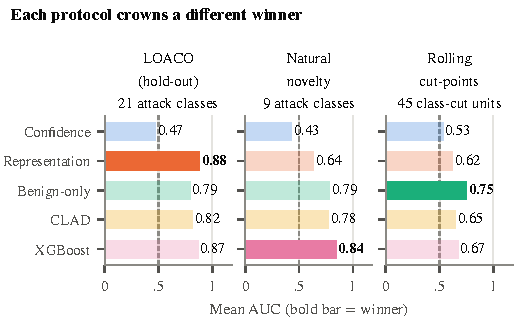
\includegraphics[width=\columnwidth]{fig_winners.pdf}
\caption{Mean AUC per detector family pooled over all classes of each protocol (rolling: all 45 class--cut units). The winner (solid bar) differs in each protocol; XGBoost is included as a supervised reference.}
\label{fig:winners}

\end{center}
\makeatother

\makeatletter
\begin{center}
\footnotesize
\setlength{\tabcolsep}{2.4pt}

\def\@captype{table}
\caption{Family mean AUC (five seeds). Bold: leading novelty family. Conf.\ = confidence, Repr.\ = representation, Benign = benign-only. Classes per evaluation in parentheses.}
\label{tab:fam}

\begin{tabular}{lccccc}
\toprule
Evaluation & Conf. & Repr. & Benign & CLAD & XGB\\
\midrule
LOACO D1 (6) & .553 & \textbf{.729} & .660 & .653 & .682\\
LOACO D2 (8) & .439 & \textbf{.977} & .807 & .949 & .998\\
LOACO D3 (6) & .426 & .881 & \textbf{.903} & .780 & .862\\
Purged D5 (1) & .580 & \textbf{.998} & .833 & .972 & 1.00\\
Natural D1 (2) & .529 & \textbf{.623} & .505 & .574 & .523\\
Natural D3 (5) & .467 & .522 & \textbf{.898} & .823 & .923\\
Natural D5 (2) & .256 & \textbf{.940} & .794 & .864 & .968\\
\bottomrule
\end{tabular}
\end{center}
\makeatother

\subsection{RQ3: Does natural novelty expose instability that hold-out evidence hides?}
\label{sec:c3}
A change of best detector could still be a matter of noise, so the third question is how much results vary across seeds, and whether LOACO reveals that variation. On the first backbone, every stochastic supervised score (the six backbone scores and CLAD) is less stable under natural novelty than under LOACO (Table~\ref{tab:sd}). The effect is smaller on the GRU: its representation scores become 2.6$\times$ less stable, its confidence scores 1.0--1.3$\times$. Seeding XGBoost (XGBoost-s) raises its seed standard deviation only to 0.014, so the instability belongs to learned representations under shift rather than to seeding as such, and its size depends on the backbone. The seeded benign-only detectors (Isolation Forest, autoencoder) stay below 0.018 seed standard deviation under natural novelty, below every supervised score's minimum of 0.074; On D3 natural novelty, $k$NN has a seed standard deviation of 0.33--0.40 AUC on four of five classes, so the same detector can rank first or last depending on the seed. Fig.~\ref{fig:d3} shows this on the three D3 classes evaluated under both protocols.

\textbf{Answer to RQ3.} Yes: natural novelty raises the seed variability of every stochastic supervised score, by up to 17$\times$ on AHSD and 2.6$\times$ for the GRU's representation scores.

\makeatletter
\begin{center}
\footnotesize
\setlength{\tabcolsep}{4pt}

\def\@captype{table}
\caption{Mean seed standard deviation of AUC. LOACO pools D1--D3; natural novelty pools D1, D3, D5. GRU rows: second backbone; XGBoost-s: seeded XGBoost.}
\label{tab:sd}

\begin{tabular}{llccc}
\toprule
Detector & Family & LOACO & Natural & Ratio\\
\midrule
MSP & Conf. & 0.061 & 0.103 & 1.7$\times$\\
Energy & Conf. & 0.055 & 0.100 & 1.8$\times$\\
$P(\text{attack})^\dagger$ & Conf. & 0.042 & 0.082 & 2.0$\times$\\
Stress & Repr. & 0.019 & 0.110 & 5.8$\times$\\
Mahalanobis & Repr. & 0.009 & 0.074 & 7.9$\times$\\
$k$NN & Repr. & 0.013 & 0.215 & 17.0$\times$\\
GRU Mahal. & Repr. & 0.008 & 0.022 & 2.6$\times$\\
GRU $k$NN & Repr. & 0.019 & 0.051 & 2.6$\times$\\
GRU MSP & Conf. & 0.049 & 0.062 & 1.3$\times$\\
GRU $P(\text{attack})$ & Conf. & 0.027 & 0.027 & 1.0$\times$\\
CLAD & Contr. & 0.020 & 0.058 & 2.9$\times$\\
XGBoost-s & Ref. & 0.006 & 0.014 & 2.4$\times$\\
Isolation Forest & Benign & 0.007 & 0.008 & 1.1$\times$\\
Autoencoder & Benign & 0.002 & 0.017 & 9.2$\times$\\
\bottomrule
\end{tabular}
\end{center}
\makeatother

\makeatletter
\begin{center}

\def\@captype{figure}
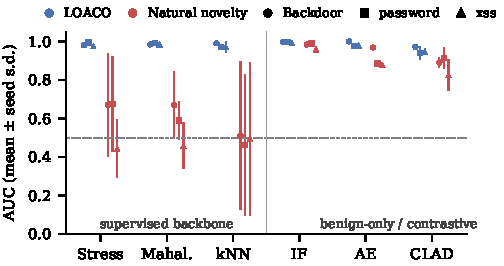
\includegraphics[width=\columnwidth]{fig_d3.pdf}
\caption{D3 (ToN-IoT) classes evaluated under both protocols: mean AUC $\pm$ seed standard deviation over five seeds. Supervised-backbone scores are tight under LOACO and spread widely under natural novelty; benign-only detectors stay tight. Dashed line: chance.}
\label{fig:d3}

\end{center}
\makeatother

\subsection{RQ4: Are confidence-based novelty scores valid in binary detectors?}
\label{sec:c4}
The confidence family scored worst in Table~\ref{tab:fam}, and Sec.~\ref{sec:method} (Stage~3) predicted why. MSP and energy fall below 0.5 wherever the classifier detects unseen attacks confidently (Table~\ref{tab:conf}). On LOACO D2, MSP is below 0.5 on every seed of all eight classes while $P(\text{attack})$ reaches 0.997--1.000 on the same models: the classifier detects the held-out attacks, and MSP reads that confidence as normality. The GRU repeats the pattern (LOACO D2: MSP 0.162 vs $P(\text{attack})$ 0.999; natural novelty D3: 0.245 vs 0.918). Across all 34 evaluation--backbone pairs, MSP exceeds $P(\text{attack})$ only in five rolling cuts where $P(\text{attack})$ is itself at or near chance (0.345--0.548), i.e.\ where the classifier misses the novel class. $P(\text{attack})$ falls below 0.5 only on individual classes (D3 LOACO ddos 0.35 and scanning 0.46; D5 portscan 0.16). Representation distance is valid on average, but on natural novelty D3 its interval [0.402, 0.647] includes 0.5.

\textbf{Answer to RQ4.} Not MSP and energy: the attack probability and representation distance are valid on average; maximum-softmax and energy invert in binary detectors on both backbones.

\makeatletter
\begin{center}
\footnotesize
\setlength{\tabcolsep}{4pt}

\def\@captype{table}
\caption{Mean AUC of confidence scores and the representation family.}
\label{tab:conf}

\begin{tabular}{lcccc}
\toprule
Evaluation & MSP & Energy & $P(\text{attack})^\dagger$ & Repr.\\
\midrule
LOACO D2 & 0.163 & 0.155 & 0.999 & 0.977\\
LOACO D3 & 0.269 & 0.258 & 0.752 & 0.881\\
Natural D3 & 0.262 & 0.287 & 0.853 & 0.522\\
Natural D5 & 0.103 & 0.090 & 0.575 & 0.940\\
\bottomrule
\end{tabular}
\end{center}
\makeatother

\subsection{RQ5: Does temporal shift alone explain the disagreement?}
\label{sec:c5}
Natural novelty mixes a new attack class with temporal shift, so this question isolates the shift itself by comparing in-distribution AUC on the grouped and temporal splits. Its effects are dataset-specific (Table~\ref{tab:temp}). On D1 both models lose 0.27--0.29 AUC under the temporal split; on D2 neither changes by more than 0.014; and on D5 both improve. Only on D3 does the AHSD backbone degrade (0.664, seed s.d.\ 0.202) while XGBoost holds 0.978; the GRU degrades less (0.981$\rightarrow$0.857), so the size of this drop depends on the backbone. Across 108 zero-shot transfer cells (12 detectors $\times$ 9 source--target pairs among D1--D4), the median AUC is 0.500 and 67\% fall in [0.3, 0.6]. Checkpoint choice moves representation and CLAD family means by at most 0.073 and confidence scores by up to 0.205 (D5, 26 validation attack windows).

\textbf{Answer to RQ5.} No: the effect of a time split depends on the dataset and the backbone, and on D5 in-distribution AUC rises under the time split while natural-novelty AUC falls (Table~\ref{tab:agree}); zero-shot transfer to a new network is near chance.

\begin{table}[!t]
\centering\footnotesize\setlength{\tabcolsep}{4pt}
\caption{In-distribution AUC, grouped vs.\ temporal split.}
\label{tab:temp}
\begin{tabular}{lcccc}
\toprule
 & \multicolumn{2}{c}{$P(\text{attack})^\dagger$} & \multicolumn{2}{c}{XGBoost}\\
\cmidrule(lr){2-3}\cmidrule(lr){4-5}
Dataset & Grouped & Temporal & Grouped & Temporal\\
\midrule
D1 & 0.812 & 0.521 & 0.815 & 0.547\\
D2 & 0.999 & 0.997 & 0.998 & 0.984\\
D3 & 0.975 & 0.664 & 0.977 & 0.978\\
D5 & 0.831 & 0.948 & 0.705 & 0.990\\
\bottomrule
\end{tabular}
\end{table}

\subsection{RQ6: Does AUC overstate operational detection?}
\label{sec:c6}
An operator does not experience AUC but the share of attacks caught at a false-alarm rate the security team can absorb; base rates make this gap well known in principle~\cite{arp2022,apruzzese2023sok}, and some zero-day studies report recall at a fixed FPR~\cite{nayak2026,mesca2026}. Here we quantify it across protocols. The two disagree sharply (Fig.~\ref{fig:operating}). Under LOACO D2 the best families catch 87--99\% of held-out windows at 1\% false-positive rate. Under natural novelty D3, benign-only detectors reach an AUC of 0.90 but catch 12\%, and XGBoost 38\%. Over the 45 rolling class--cut units no family exceeds 18\% (XGBoost 0.18; benign-only 0.09 at AUC 0.75), and of the 333 detector--class points with AUC $\geq0.75$ under natural novelty, 184 catch fewer than 20\% of attack windows (median 0.15): novel attacks overlap the benign score tail.

\textbf{Answer to RQ6.} Yes: over the rolling cuts, family AUCs up to 0.75 catch at most 18\% of new attacks at a 1\% false-positive rate.

\makeatletter
\begin{center}

\def\@captype{figure}
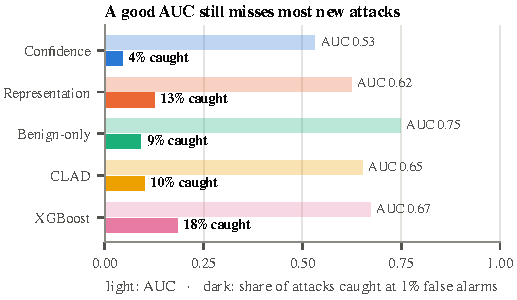
\includegraphics[width=\columnwidth]{fig_operating.pdf}
\caption{Rolling cut-points (45 class--cut units): each family's AUC (light bar) against the share of novel attack windows it catches at 1\% false-positive rate (dark bar).}
\label{fig:operating}

\end{center}
\makeatother

\textbf{Comparison with published results.} Class hold-out results in the literature (AUROC 0.971--0.997~\cite{wilkie2026,nayak2026}; 87--92\% zero-day detection~\cite{sarhan2023zeroshot}) are matched by HoNE's LOACO numbers on D2 and D5, but the same detectors drop under natural novelty and rolling cuts (CLAD: 0.972 on purged D5, 0.702 rolling; rolling TPR@1\% $\leq$0.18 against a published recall@1\%FPR of 0.783~\cite{nayak2026}); published softmax and energy AUROCs of 0.76--0.80 on multi-class NF-ToN-IoT~\cite{talpini2024} contrast with 0.269 and 0.258 in our binary detectors.

\subsection{Pre-registered negative results}
\label{sec:neg}
Four confirmatory hypotheses were tested against frozen gates, and all four failed: a spectral model of per-class detectability (pooled $\rho{=}0.326$, below 0.6); attack absorption by an adaptive equilibrium under supervised training (not reproduced; detectability peaks at a small adaptation rate); benign-drift re-anchoring (0 of 9 detectors met the improvement criterion); and benign-only superiority confined to natural novelty. The last gate's supervised family included MSP and energy, which Sec.~\ref{sec:c4} shows are invalid; the verdict stands as recorded. The descriptive findings were recorded after these failures, under hashed amendments, not selected to fit a narrative.

\section{Discussion}
\label{sec:disc}
\textbf{Protocol validity, not a new benchmark.} HoNE is not proposed as a new detector benchmark; it treats the evaluation protocol as the object of study and asks whether conclusions drawn under the conventional protocol survive under the conditions that protocol is meant to represent. The agreement analysis answers in measurable terms: LOACO's family-level signal survives, but its detector choice, ranking, absolute AUC, stability and operating point do not.

\textbf{Interpretation.} The findings have a common cause: the protocols disagree because they change different things. LOACO keeps the benign traffic of the test period in training, so supervised representations place a held-out class far from benign traffic and distance scores excel (0.977 on D2). Under natural novelty the benign traffic itself shifts and representations shaped by known attacks lose their reference point, explaining the drop and the seed dependence on D3 (less on the GRU: 0.869). Benign-only detectors never see attacks, which explains their stability but not their accuracy: they lead on D3 natural novelty yet trail by 0.17 AUC on D2 LOACO. XGBoost's strength matches evidence that tree ensembles are hard to beat on tabular data~\cite{grinsztajn2022}, but its collapse at some cut-points shows that a supervised boundary can misplace a new class.

\label{sec:protocol}
\textbf{What works: the HoNE acceptance protocol.} Each check is derived as finding $\rightarrow$ failure mode $\rightarrow$ required evidence, so that an operator can see why it is needed before trusting a zero-day claim:
\begin{enumerate}
\item \textbf{Leakage controls stated.} Random splits share flows and attack episodes between training and test~\cite{arp2022}; require time-block grouping before windowing, window deduplication and purging for short captures.
\item \textbf{Natural novelty next to LOACO.} The best detector changed in 11 of 12 paired comparisons (Sec.~\ref{sec:c2}), so LOACO alone cannot select a detector; require natural-novelty results at several cut-points wherever timestamps allow, and a statement when a protocol is infeasible (Sec.~\ref{sec:c1}).
\item \textbf{Five or more seeds.} Natural novelty raises seed variation by up to 17$\times$ (Sec.~\ref{sec:c3}), so one run can misrank detectors; require per-class seed standard deviations, not only means.
\item \textbf{Valid novelty scores.} MSP and energy rank detected attacks as normal in binary detectors (Sec.~\ref{sec:c4}); require $P(\text{attack})$ or a representation distance validated under natural novelty.
\item \textbf{Two baselines.} XGBoost or the benign-only family matched or exceeded every other family in five of seven fixed evaluations, and benign-only detectors led over the rolling cut-points (Sec.~\ref{sec:c2}); require both a benign-only detector and a gradient-boosted tree.
\item \textbf{Operating-point metrics.} AUCs up to 0.75 caught at most 18\% of new attacks at 1\% FPR (Sec.~\ref{sec:c6}); require TPR at the false-positive rate the security team can absorb.
\item \textbf{Checkpoint sensitivity.} Checkpoint choice moved confidence scores by up to 0.205 on D5's small validation set (Sec.~\ref{sec:c5}); require it when validation sets are small.
\item \textbf{Pre-registration or a full amendment log}, including failed hypotheses (Sec.~\ref{sec:neg}), so that reported findings can be told apart from selected ones.
\end{enumerate}
If a check is unmet, the operator should request the missing evidence.

\textbf{Remaining limitations.} Both backbones are recurrent, and effect sizes already differ between them, so the findings describe the evaluated detectors under these protocols, not learned NIDS in general; what they establish is that evaluation conclusions depend on the protocol. D1 and D5 contribute two natural-novelty classes each in the primary split; the rolling cuts add 45 class--cut units, but units of one class at several cuts share test windows and are not independent. Grouping, labelling and threshold choices were fixed in advance but are not the only reasonable ones; $P(\text{attack})$ was added post hoc; and CLAD was reimplemented from its paper (0.972 on purged D5 against the 0.997 its authors report on a random split~\cite{wilkie2026}). Natural novelty is novel \emph{behaviour}; many real zero-days exploit new vulnerabilities with familiar behaviour~\cite{jibunoh2026}, which no flow benchmark captures. Finally, all datasets come from testbeds: natural novelty follows the capture schedule, closer to deployment than LOACO but not live traffic.

\section{Conclusion}
\label{sec:concl}
HoNE tested whether LOACO evidence stands for the new attacks an operator will face, and found that it does not: LOACO could not be run on day-scheduled captures, the best detector changed in 11 of 12 paired comparisons, seed variability rose up to 17$\times$, and AUCs up to 0.75 caught at most 18\% of new attacks at 1\% FPR. Each failure yields one of eight acceptance checks, and HoNE's released splits and code let any zero-day claim be tested under both protocols.

\section*{Artifacts}
All code, splits, amendment logs and the result files behind every number in this paper are available at \artifact.

\clearpage
\bibliographystyle{IEEEtran}
\begin{thebibliography}{40}

\bibitem{wilkie2026}
J.~Wilkie, H.~Hindy, C.~Michie, C.~Tachtatzis, J.~Irvine, and R.~Atkinson, ``A novel contrastive loss for zero-day network intrusion detection,'' \emph{IEEE Trans. Netw. Service Manag.}, vol.~23, pp. 2064--2076, 2026.

\bibitem{jodayree2026}
M.~Jodayree, A.~Kavoosi~Ghafi, S.~Amiri, and P.~Shaykholeslami, ``Explainable zero-day attack detection in IoMT using transformer-based time-series modeling,'' \emph{Sci. Rep.}, vol.~16, Art. no. 23252, 2026.

\bibitem{arp2022}
D.~Arp, E.~Quiring, F.~Pendlebury, A.~Warnecke, F.~Pierazzi, C.~Wressnegger, L.~Cavallaro, and K.~Rieck, ``Dos and don'ts of machine learning in computer security,'' in \emph{Proc. 31st USENIX Security Symp.}, 2022, pp. 3971--3988.

\bibitem{engelen2021}
G.~Engelen, V.~Rimmer, and W.~Joosen, ``Troubleshooting an intrusion detection dataset: The CICIDS2017 case study,'' in \emph{Proc. IEEE Security and Privacy Workshops (SPW)}, 2021, pp. 7--12.

\bibitem{hendrycks2017}
D.~Hendrycks and K.~Gimpel, ``A baseline for detecting misclassified and out-of-distribution examples in neural networks,'' in \emph{Proc. Int. Conf. Learn. Represent. (ICLR)}, 2017.

\bibitem{liu2020energy}
W.~Liu, X.~Wang, J.~Owens, and Y.~Li, ``Energy-based out-of-distribution detection,'' in \emph{Proc. Adv. Neural Inf. Process. Syst. (NeurIPS)}, 2020, pp. 21\,464--21\,475.

\bibitem{sommer2010}
R.~Sommer and V.~Paxson, ``Outside the closed world: On using machine learning for network intrusion detection,'' in \emph{Proc. IEEE Symp. Security and Privacy (S\&P)}, 2010, pp. 305--316.

\bibitem{apruzzese2023sok}
G.~Apruzzese, P.~Laskov, and J.~Schneider, ``SoK: Pragmatic assessment of machine learning for network intrusion detection,'' in \emph{Proc. IEEE European Symp. Security and Privacy (EuroS\&P)}, 2023, pp. 592--614.

\bibitem{rosay2021}
A.~Rosay, F.~Carlier, E.~Cheval, and P.~Leroux, ``From CIC-IDS2017 to LYCOS-IDS2017: A corrected dataset for better performance,'' in \emph{Proc. IEEE/WIC/ACM Int. Conf. Web Intell. Intell. Agent Technol. (WI-IAT)}, 2021, pp. 570--575.

\bibitem{pinto2025}
D.~Pinto, I.~Amorim, E.~Maia, and I.~Pra\c{c}a, ``A review on intrusion detection datasets: Tools, processes, and features,'' \emph{Comput. Netw.}, vol.~262, Art. no. 111177, 2025.

\bibitem{sarhan2021netflow}
M.~Sarhan, S.~Layeghy, N.~Moustafa, and M.~Portmann, ``NetFlow datasets for machine learning-based network intrusion detection systems,'' in \emph{Big Data Technologies and Applications (BDTA 2020)}, LNICST, vol.~371. Springer, 2021, pp. 117--135.

\bibitem{sarhan2022standard}
M.~Sarhan, S.~Layeghy, and M.~Portmann, ``Towards a standard feature set for network intrusion detection system datasets,'' \emph{Mobile Netw. Appl.}, vol.~27, no.~1, pp. 357--370, 2022.

\bibitem{luay2025}
M.~Luay, S.~Layeghy, N.~Noorbin, M.~Sarhan, G.~Kulatilleke, N.~Moustafa, and M.~Portmann, ``Time matters: Temporal NetFlow features for ML-based network intrusion detection,'' \emph{IEEE Access}, vol.~14, pp. 66899--66913, 2026.

\bibitem{zoppi2023}
T.~Zoppi, A.~Ceccarelli, T.~Puccetti, and A.~Bondavalli, ``Which algorithm can detect unknown attacks? Comparison of supervised, unsupervised and meta-learning algorithms for intrusion detection,'' \emph{Comput. Secur.}, vol.~127, Art. no. 103107, 2023.

\bibitem{sarhan2023zeroshot}
M.~Sarhan, S.~Layeghy, M.~Gallagher, and M.~Portmann, ``From zero-shot machine learning to zero-day attack detection,'' \emph{Int. J. Inf. Secur.}, vol.~22, no.~4, pp. 947--959, 2023.

\bibitem{layeghy2023xdomain}
S.~Layeghy and M.~Portmann, ``Explainable cross-domain evaluation of ML-based network intrusion detection systems,'' \emph{Comput. Electr. Eng.}, vol.~108, Art. no. 108692, 2023.

\bibitem{layeghy2023dinids}
S.~Layeghy, M.~Baktashmotlagh, and M.~Portmann, ``DI-NIDS: Domain invariant network intrusion detection system,'' \emph{Knowl.-Based Syst.}, vol.~273, Art. no. 110626, 2023.

\bibitem{martinez2026}
B.~A. Mart\'{\i}nez Gonz\'{a}lez, A.~D. Bermejo, M.~P\'{e}rez Sevilla, J.~A. Rinc\'{o}n Arango, and D.~Urda, ``Cross-domain generalization strategies for IoT cyberattack detection using flow-based features,'' \emph{Internet Things}, vol.~39, Art. no. 102044, 2026.

\bibitem{sharafaldin2018}
I.~Sharafaldin, A.~H. Lashkari, and A.~A. Ghorbani, ``Toward generating a new intrusion detection dataset and intrusion traffic characterization,'' in \emph{Proc. 4th Int. Conf. Inf. Syst. Secur. Privacy (ICISSP)}, 2018, pp. 108--116.

\bibitem{moustafa2015}
N.~Moustafa and J.~Slay, ``UNSW-NB15: A comprehensive data set for network intrusion detection systems,'' in \emph{Proc. Military Commun. Inf. Syst. Conf. (MilCIS)}, 2015, pp. 1--6.

\bibitem{moustafa2021}
N.~Moustafa, ``A new distributed architecture for evaluating AI-based security systems at the edge: Network TON\_IoT datasets,'' \emph{Sustain. Cities Soc.}, vol.~72, Art. no. 102994, 2021.

\bibitem{koroniotis2019}
N.~Koroniotis, N.~Moustafa, E.~Sitnikova, and B.~Turnbull, ``Towards the development of realistic botnet dataset in the Internet of Things for network forensic analytics: Bot-IoT dataset,'' \emph{Future Gener. Comput. Syst.}, vol.~100, pp. 779--796, 2019.

\bibitem{lopezdeprado2018}
M.~L\'{o}pez de Prado, \emph{Advances in Financial Machine Learning}. Hoboken, NJ, USA: Wiley, 2018.

\bibitem{yang2024ood}
J.~Yang, K.~Zhou, Y.~Li, and Z.~Liu, ``Generalized out-of-distribution detection: A survey,'' \emph{Int. J. Comput. Vis.}, vol.~132, no.~12, pp. 5635--5662, 2024.

\bibitem{lee2018}
K.~Lee, K.~Lee, H.~Lee, and J.~Shin, ``A simple unified framework for detecting out-of-distribution samples and adversarial attacks,'' in \emph{Proc. Adv. Neural Inf. Process. Syst. (NeurIPS)}, vol.~31, 2018.

\bibitem{sun2022knn}
Y.~Sun, Y.~Ming, X.~Zhu, and Y.~Li, ``Out-of-distribution detection with deep nearest neighbors,'' in \emph{Proc. 39th Int. Conf. Mach. Learn. (ICML)}, 2022, pp. 20\,827--20\,840.

\bibitem{liu2008}
F.~T. Liu, K.~M. Ting, and Z.-H. Zhou, ``Isolation forest,'' in \emph{Proc. 8th IEEE Int. Conf. Data Mining (ICDM)}, 2008, pp. 413--422.

\bibitem{scholkopf2001}
B.~Sch\"{o}lkopf, J.~C. Platt, J.~Shawe-Taylor, A.~J. Smola, and R.~C. Williamson, ``Estimating the support of a high-dimensional distribution,'' \emph{Neural Comput.}, vol.~13, no.~7, pp. 1443--1471, 2001.

\bibitem{chen2016}
T.~Chen and C.~Guestrin, ``XGBoost: A scalable tree boosting system,'' in \emph{Proc. 22nd ACM SIGKDD Int. Conf. Knowl. Discov. Data Min. (KDD)}, 2016, pp. 785--794.

\bibitem{nosek2018}
B.~A. Nosek, C.~R. Ebersole, A.~C. DeHaven, and D.~T. Mellor, ``The preregistration revolution,'' \emph{Proc. Natl. Acad. Sci. USA}, vol.~115, no.~11, pp. 2600--2606, 2018.

\bibitem{grinsztajn2022}
L.~Grinsztajn, E.~Oyallon, and G.~Varoquaux, ``Why do tree-based models still outperform deep learning on typical tabular data?'' in \emph{Proc. Adv. Neural Inf. Process. Syst. (NeurIPS), Datasets and Benchmarks Track}, vol.~35, 2022, pp. 507--520.

\bibitem{mirsky2018}
Y.~Mirsky, T.~Doitshman, Y.~Elovici, and A.~Shabtai, ``Kitsune: An ensemble of autoencoders for online network intrusion detection,'' in \emph{Proc. Netw. Distrib. Syst. Secur. Symp. (NDSS)}, 2018.

\bibitem{fernandez2026}
E.~Fern\'{a}ndez-Morales, J.~C. Garc\'{\i}a-Merino, L.~Tobarra, A.~Robles-G\'{o}mez, and R.~Pastor-Vargas, ``Deep learning approaches for intrusion detection in IoT environments: A systematic literature review,'' \emph{IEEE Internet Things J.}, vol.~13, no.~20, pp. 46485--46513, Oct. 2026.

\bibitem{manocchio2024}
L.~D. Manocchio, S.~Layeghy, W.~W. Lo, G.~K. Kulatilleke, M.~Sarhan, and M.~Portmann, ``FlowTransformer: A transformer framework for flow-based network intrusion detection systems,'' \emph{Expert Syst. Appl.}, vol.~241, Art. no. 122564, 2024.

\bibitem{wang2024snn}
Z.~Wang, F.~A. Ghaleb, A.~Zainal, M.~M. Siraj, and X.~Lu, ``An efficient intrusion detection model based on convolutional spiking neural network,'' \emph{Sci. Rep.}, vol.~14, Art. no. 7054, 2024.

\bibitem{knapp2025}
L.~Knapp, S.~Nitzsche, M.~B\"{o}rsig, A.~Vasilache, I.~Baumgart, and J.~Becker, ``Efficacy of spiking neural networks for intrusion detection systems,'' in \emph{Proc. Int. Conf. Cybersecurity and AI-Based Systems (Cyber-AI)}, 2025, pp. 89--95.

\bibitem{liu2026netmasq}
Z.~Liu, Y.~Zhao, Z.~Liu, Q.~Li, C.~Fu, G.~Zhou, and K.~Xu, ``A hard-label black-box evasion attack against ML-based malicious traffic detection systems,'' in \emph{Proc. Netw. Distrib. Syst. Secur. Symp. (NDSS)}, 2026.

\bibitem{xu2026entente}
J.~Xu, C.~Li, Y.~Zheng, and Z.~Li, ``Entente: Cross-silo intrusion detection on network log graphs with federated learning,'' in \emph{Proc. Netw. Distrib. Syst. Secur. Symp. (NDSS)}, 2026.

\bibitem{depaola2026}
A.~De~Paola, S.~Drago, P.~Ferraro, and G.~Lo~Re, ``HOIDS: Concept drift aware hybrid online intrusion detection system,'' \emph{J. Netw. Comput. Appl.}, vol.~254, Art. no. 104556, 2026.

\bibitem{yang2021cade}
L.~Yang, W.~Guo, Q.~Hao, A.~Ciptadi, A.~Ahmadzadeh, X.~Xing, and G.~Wang, ``CADE: Detecting and explaining concept drift samples for security applications,'' in \emph{Proc. 30th USENIX Security Symp.}, 2021, pp. 2327--2344.

\bibitem{nayak2026}
S.~Nayak, ``ThreatFormer-IDS: Robust transformer intrusion detection with zero-day generalization and explainable attribution,'' arXiv:2603.00185, 2026.

\bibitem{alhalangy2026}
A.~Alhalangy and G.~A. Eltayeb, ``Drift-aware continual generative behavioral detection for zero-day cyberattacks: Reproducible temporal evaluation and SIEM-ready alerting,'' \emph{Information}, vol.~17, no.~9, Art. no. 852, 2026.

\bibitem{mesca2026}
S.~Mesca, E.~Pricop, and G.~Stamatescu, ``Rigorous evaluation of machine learning intrusion detection for water treatment systems on SWaT network traffic,'' \emph{Appl. Sci.}, vol.~16, no.~14, Art. no. 7206, 2026.

\bibitem{raj2026}
M.~Raj, H.~Tyagi, and A.~Kaur, ``A leakage-safe re-evaluation of machine-learning intrusion detection for RPL-based IoT networks,'' \emph{J. Eng. Res.}, 2026, doi: 10.1016/j.jer.2026.09.059.

\bibitem{sakr2026}
H.~A. Sakr \emph{et al.}, ``Explainable and deployment-aware zero-day intrusion detection for cloud-level backend and management ecosystems in EV/V2X cyber--physical systems,'' \emph{Computers}, vol.~15, no.~9, Art. no. 599, 2026.

\bibitem{youssef2026}
M.~A. Youssef, ``Stream assembly is an uncontrolled treatment in streaming intrusion-detection benchmarks,'' arXiv:2605.24696, 2026.

\bibitem{moczkodan2026}
Z.~Moczkodan and H.~Ragab, ``Do transformers actually help intrusion detection? A temporal sequence evaluation on CIC-IDS2017,'' arXiv:2606.11098, 2026.

\bibitem{abdessamad2026}
M.~Abdessamad and E.~B. Tazi, ``Feature selection versus feature extraction for IoT intrusion detection under temporal evaluation,'' \emph{Int. J. Adv. Comput. Sci. Appl.}, vol.~17, no.~8, 2026.

\bibitem{pendlebury2019}
F.~Pendlebury, F.~Pierazzi, R.~Jordaney, J.~Kinder, and L.~Cavallaro, ``TESSERACT: Eliminating experimental bias in malware classification across space and time,'' in \emph{Proc. 28th USENIX Security Symp.}, 2019, pp. 729--746.

\bibitem{andresini2021}
G.~Andresini, F.~Pendlebury, F.~Pierazzi, C.~Loglisci, A.~Appice, and L.~Cavallaro, ``INSOMNIA: Towards concept-drift robustness in network intrusion detection,'' in \emph{Proc. 14th ACM Workshop Artif. Intell. Secur. (AISec)}, 2021, pp. 111--122.

\bibitem{dragoi2022}
M.~Dragoi, E.~Burceanu, E.~Haller, A.~Manolache, and F.~Brad, ``AnoShift: A distribution shift benchmark for unsupervised anomaly detection,'' in \emph{Proc. Adv. Neural Inf. Process. Syst. (NeurIPS), Datasets and Benchmarks Track}, vol.~35, 2022, pp. 32854--32867.

\bibitem{schraven2026}
J.~Schraven, A.~Windmann, and O.~Niggemann, ``MAWIFlow benchmark: Realistic flow-based evaluation for network intrusion detection,'' in \emph{Proc. 12th Int. Conf. Inf. Syst. Secur. Privacy (ICISSP)}, 2026, pp. 549--556.

\bibitem{corsini2023}
A.~Corsini and S.~J. Yang, ``Are existing out-of-distribution techniques suitable for network intrusion detection?'' in \emph{Proc. IEEE Conf. Commun. Netw. Secur. (CNS)}, 2023, pp. 1--9.

\bibitem{zhang2021}
Z.~Zhang, Y.~Zhang, D.~Guo, and M.~Song, ``A scalable network intrusion detection system towards detecting, discovering, and learning unknown attacks,'' \emph{Int. J. Mach. Learn. Cybern.}, vol.~12, no.~6, pp. 1649--1665, 2021.

\bibitem{talpini2024}
J.~Talpini, F.~Sartori, and M.~Savi, ``Enhancing trustworthiness in ML-based network intrusion detection with uncertainty quantification,'' \emph{J. Reliable Intell. Environ.}, vol.~10, no.~4, pp. 501--520, 2024.

\bibitem{baye2023}
G.~Baye, P.~Silva, A.~Broggi, L.~Fiondella, N.~D. Bastian, and G.~Kul, ``Performance analysis of deep-learning based open set recognition algorithms for network intrusion detection systems,'' in \emph{Proc. IEEE/IFIP Netw. Oper. Manag. Symp. (NOMS)}, 2023, pp. 1--6.

\bibitem{cantone2024}
M.~Cantone, C.~Marrocco, and A.~Bria, ``Machine learning in network intrusion detection: A cross-dataset generalization study,'' \emph{IEEE Access}, vol.~12, pp. 144489--144508, 2024.

\bibitem{jibunoh2026}
N.~Jibunoh, S.~Khanchi, and A.~Makanju, ``Zero day attacks: Novel behaviour or novel vulnerability?'' arXiv:2605.03138, 2026.

\end{thebibliography}

\end{document}
